%% Type de document et encodage de la police
\documentclass[a4paper]{article}
\usepackage[utf8x]{inputenc}
\usepackage[T1]{fontenc}
% \usepackage[french]{babel}

%% Initialise la taille des pages et des marges
\usepackage[a4paper, top=3cm, bottom=3cm, left=2cm, right=2cm, marginparwidth=2cm]{geometry}

%% Commandes perso
\renewcommand{\arraystretch}{1.2} %% row 20% longer

%% Pour les exemples
\usepackage{mdframed}
\newmdenv[topline=false, bottomline=false, rightline=false, skipabove=\topsep, skipbelow=\topsep]{example}

%% Pour les diagrammes
\usepackage{tikz}
\usetikzlibrary{calc}
\tikzstyle{incolore} = [rectangle, draw=black, minimum height=1cm, minimum width=3cm, text width=3cm, text centered]

%% Packs utiles
\usepackage{amsmath}
\usepackage{graphicx}
\usepackage{fancyvrb}
\usepackage{colortbl}


\title{Bases de Données}
\author{Grégoire Roumache}
\date{Avril 2020}

\begin{document}

\maketitle















\section{Configuration SQL Server}





\begin{itemize}





\item Activer SQL Server:
\begin{enumerate}
    \item Dans la barre de recherche Windows, taper: \textit{services.msc}.
    \item Aller à \textit{SQL Server (sqlexpress)} et activer le service. Le reste peut être désactivé.
\end{enumerate}





\item Créer une base de données:
\begin{enumerate}
    \item Ouvrir \textit{SQL Server Management Studio}.
    \item Dans le menu de gauche, en-dessous du nom de l'ordinateur, click-droit sur \textit{Databases}.
    \item Clicker sur \textit{New Database}.
    \item Donner un nom à la base de données dans \textit{Database name}.
    \item Dans le menu de gauche, clicker sur \textit{Options}.
    \item Configurer \textit{Collation} (\textit{Classement} en français) sur \textit{Latin\_General\_100\_CI\_AS}.
    \begin{example}
        \begin{itemize}
            \item CI = case insensitive
            \item AS = accent sensitive
        \end{itemize}
        \textbf{Remarque:} \textit{French\_CI\_AS} revient à peu près au même.
    \end{example}
\end{enumerate}





\end{itemize}















\section{Introduction}





\begin{itemize}



\item Qu'est-ce qu'une donnée ?
\begin{example}
    l'enregistrement dans un code donné d’un objet, un texte, un concept, un fait, etc.
\end{example}



\item Donnée $ \neq $ Information ?
\begin{example}
    l'information est le sens qu'on donne à une donnée
\end{example}



\item Une base de données, c'est:
\begin{itemize}
    \item une \textbf{collection de données en relation}
    \item \textbf{indépendante} des applications
    \item \textbf{sans redondance} inutile
    \item \textbf{partageable} entre plusieurs utilisateurs
    \item on \textbf{accéde} à son contenu \textbf{en lui posant une question}
\end{itemize}



\item SGBD = système de gestion de bases de données
\begin{example}
    Le SGBD (système de gestion de bases de données) permet de:
    \begin{itemize}
        \item \textbf{créer} et \textbf{supprimer} des fichiers
        \item \textbf{insérer}, \textbf{effacer} et \textbf{modifier} des enregistrements
        \item \textbf{rechercher} des données
    \end{itemize}
\end{example}



\item Que doit gérer un SGBD ?
\begin{example}
    \begin{itemize}
        \item Accès optimal à toutes les données
        \item Traitement simultané des données
        \item Validité et cohérence des données
        \item Sécurité des données
        \item Sauvegarde et récupération
    \end{itemize}
\end{example}



\end{itemize}















\section{Schéma conceptuel}










\subsection{Entité-relation}





\begin{itemize}



\item but du schéma conceptuel = \textbf{modéliser} un système. On y définit les concepts et les liens qui les unissent



\item entité = quelque chose lié au système que l'on veut modéliser (ex: personne, réservation, etc.)



\item attribut = caractéristique d'une entité



\item relation = lien entre les entités



\item occurence = 



\end{itemize}










\subsection{Notation}





\begin{itemize}



\item Notation d'une entité:
\begin{itemize}
    \item rectangle divisé en 2 parties,
    \item 1ère partie = nom de l'entité, en \textbf{majuscule}, au \textbf{singulier},
    \item 2ème partie = les attributs, en \textbf{CamelCase}, au \textbf{singulier}.
\end{itemize}



\item Notation d'un attribut:
\begin{itemize}
    \item un attribut \textbf{souligné} est un \textbf{identifiant},
    \item un attribut suivi de \textbf{[0-1]} est un attribut \textbf{optionnel}.
\end{itemize}



\item Notation des relations:
\begin{itemize}
    \item une relation est simplement une ligne qui relie les entités,
    \item elle a un \textbf{rôle} qui est écrit \textbf{au milieu de la ligne},
    \item elle a aussi des \textbf{cardinalités à ses extrémités}.
    \begin{example}
        une cardinalité exprime le nombre d'occurences d'une entité par rapport à une autre entité
    \end{example}
\end{itemize}



\end{itemize}



Exemple (1):
\begin{center}
    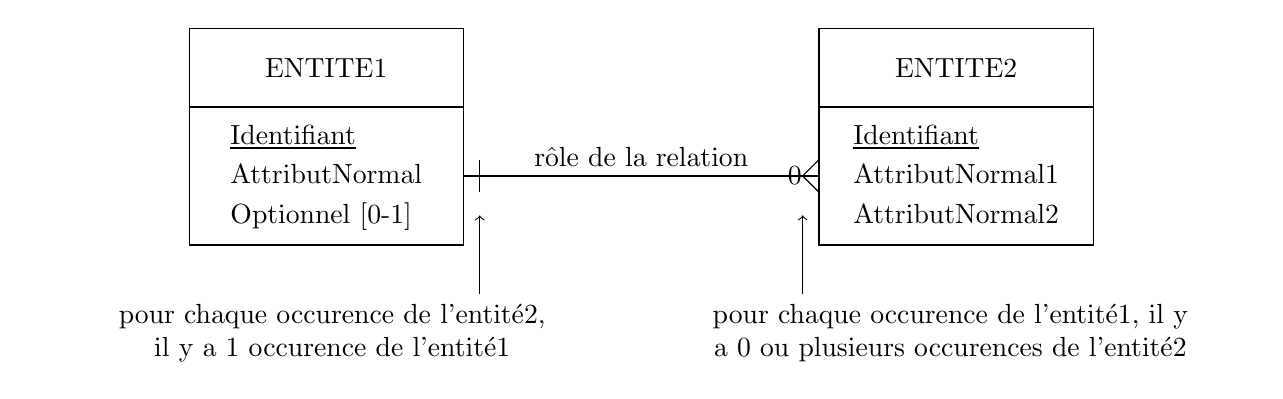
\begin{tikzpicture}

        \node () [incolore, anchor=north west, text width=3.25cm] at (0,0) {ENTITE1};
        \node (E1) [incolore, anchor=north west, text width=3.25cm] at (0,-1) {\begin{tabular}{l}
            \underline{Identifiant} \\
            AttributNormal \\
            Optionnel [0-1]
        \end{tabular}};

        \node () [incolore, anchor=north west, text width=3.25cm] at (8,0) {ENTITE2};
        \node (E2) [incolore, anchor=north west, text width=3.25cm] at (8,-1) {\begin{tabular}{l}
            \underline{Identifiant} \\
            AttributNormal1 \\
            AttributNormal2
        \end{tabular}};


        \draw (E1) -- node[anchor=south]{rôle de la relation} (E2);
        \draw ($(E1.east) + (0.2,-0.2)$) -- ($(E1.east) + (0.2,0.2)$);

        \draw ($(E2.west) + (-0.2,0)$) -- ($(E2.west) + (0,0.2)$);
        \draw ($(E2.west) + (-0.2,0)$) -- ($(E2.west) + (0,-0.2)$);
        \node [] at ($(E2.west) + (-0.3,0)$) {0};


        \draw[->] ($(E1.east) + (0.2,-1.5)$) node[anchor=north east, xshift=2cm, text width=7.5cm, text centered]{pour chaque occurence de l'entité2, il y a 1 occurence de l'entité1} -- ($(E1.east) + (0.2,-0.5)$);
        \draw[->] ($(E2.west) + (-0.2,-1.5)$) node[anchor=north west, xshift=-2cm, text width=7.5cm, text centered]{pour chaque occurence de l'entité1, il y a 0 ou plusieurs occurences de l'entité2} -- ($(E2.west) + (-0.2,-0.5)$);

    \end{tikzpicture}
\end{center}



Exemple (2):
\begin{center}
    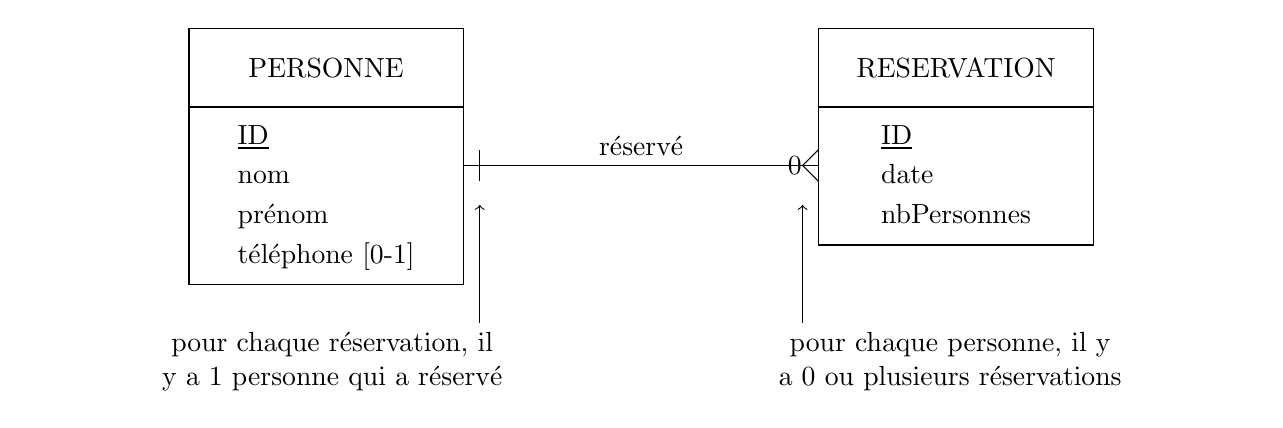
\begin{tikzpicture}

        \node () [incolore, anchor=north west, text width=3.25cm] at (0,0) {PERSONNE};
        \node (E1) [incolore, anchor=north west, text width=3.25cm] at (0,-1) {\begin{tabular}{l}
            \underline{ID} \\
            nom \\
            prénom \\
            téléphone [0-1]
        \end{tabular}};

        \node () [incolore, anchor=north west, text width=3.25cm] at (8,0) {RESERVATION};
        \node (E2) [incolore, anchor=north west, text width=3.25cm] at (8,-1) {\begin{tabular}{l}
            \underline{ID} \\
            date \\
            nbPersonnes
        \end{tabular}};


        \draw (3.5,-1.75) -- node[anchor=south]{réservé} (8,-1.75);
        \draw ($(3.5,-1.75) + (0.2,-0.2)$) -- ($(3.5,-1.75) + (0.2,0.2)$);

        \draw ($(8,-1.75) + (-0.2,0)$) -- ($(8,-1.75) + (0,0.2)$);
        \draw ($(8,-1.75) + (-0.2,0)$) -- ($(8,-1.75) + (0,-0.2)$);
        \node [] at ($(8,-1.75) + (-0.3,0)$) {0};


        \draw[->] ($(3.5,-1.75) + (0.2,-2)$) node[anchor=north east, xshift=2cm, text width=7.5cm, text centered]{pour chaque réservation, il y a 1 personne qui a réservé} -- ($(3.5,-1.75) + (0.2,-0.5)$);
        \draw[->] ($(8,-1.75) + (-0.2,-2)$) node[anchor=north west, xshift=-2cm, text width=7.5cm, text centered]{pour chaque personne, il y a 0 ou plusieurs réservations} -- ($(8,-1.75) + (-0.2,-0.5)$);

    \end{tikzpicture}
\end{center}



\textbf{Remarque:} on peut ajouter des "commentaires" dans le schéma, ce sont les \textbf{contraintes d'intégrité}. Exemple:
\begin{center}
    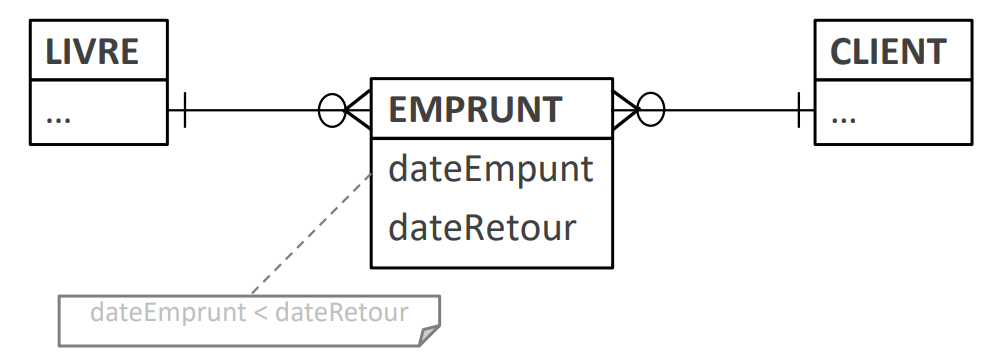
\includegraphics[width=0.7\textwidth]{../images/entite-relation02.PNG}
\end{center}










\subsection{Méthode pour créer le schéma}





\begin{enumerate}
    \item Identifier les \textbf{entités} et leur \textbf{attributs}.
    \item Souligner les attributs servant d'\textbf{identifiants} et ajouter [0-1] aux \textbf{attributs optionnels}.
    \item Identifier les \textbf{relations} entre les entités.
    \item Ajouter les \textbf{cardinalités}.
    \item Ajouter les \textbf{contraintes d'intégrité} (si nécessaire).
    \item \textbf{Vérifier} que le schéma est correct et le \textbf{normaliser} si besoin.
\end{enumerate}










\subsection{Normalisation}





\begin{itemize}



\item normalisation = ensemble de bonnes pratiques



\item La nomalisation permet d'éviter:
\begin{itemize}
    \item les contre-performances
    \item la redondance d'information
    \item les anomalies transactionnelles
\end{itemize}



\item La normalisation permet d'améliorer:
\begin{itemize}
    \item les mises à jours
    \item la maintenance
    \item l'évolution
\end{itemize}



\item Il y a 3 formes de normalisation:
\begin{enumerate}
    \item \textbf{1ère forme}:
    \begin{itemize}
        \item tous les attributs dépendent de l'identifiant,
        \item tous les attributs ont une valeur atomique.
    \end{itemize}
    \item \textbf{2ème forme}: un attribut ne peut pas dépendre d'une seule partie de l'identifiant.
    \item \textbf{3ème forme}: aucun attribut ne peut dépendre d'un autre attribut à l'execption de l'identifiant.
\end{enumerate}



\item Exemples de normalisation:
\begin{enumerate}

    \item 1ère forme:
    \begin{example}
        \begin{center}
            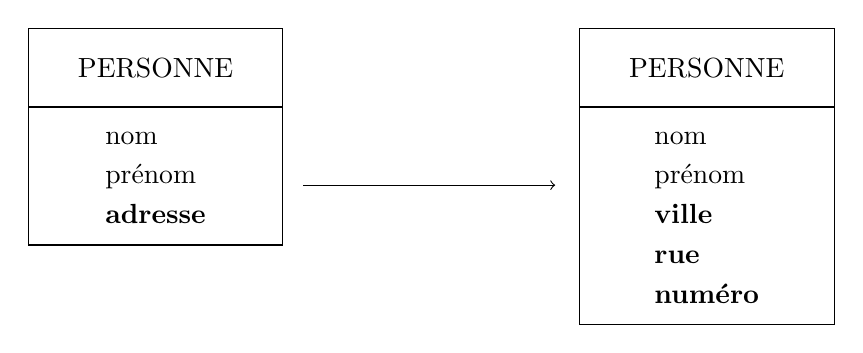
\begin{tikzpicture}
                \node [incolore, anchor=north west] at (0,0) {PERSONNE};
                \node [incolore, anchor=north west] at (0,-1) {\begin{tabular}{l}
                    nom \\
                    prénom \\
                    \textbf{adresse}
                \end{tabular}};

                \node [incolore, anchor=north west] at (7,0) {PERSONNE};
                \node [incolore, anchor=north west] at (7,-1) {\begin{tabular}{l}
                    nom \\
                    prénom \\
                    \textbf{ville} \\
                    \textbf{rue} \\
                    \textbf{numéro}
                \end{tabular}};

                \draw[->] (3.5,-2) -- (6.7,-2);
            \end{tikzpicture}
        \end{center}
        L'attribut \textbf{adresse} n'a pas une valeur atomique donc on la sépare en ses composants.
    \end{example}

    \item 2ème forme:
    \begin{example}
        \begin{center}
            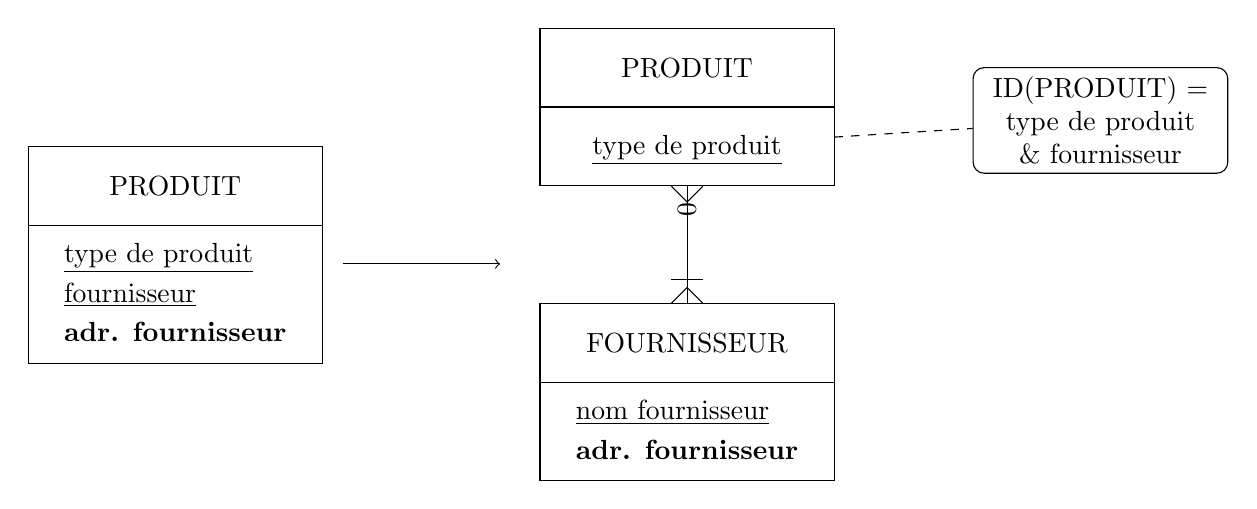
\begin{tikzpicture}
                \node [incolore, anchor=north west, text width=3.5cm] at (0,-1.5) {PRODUIT};
                \node [incolore, anchor=north west, text width=3.5cm] at (0,-2.5) {\begin{tabular}{l}
                    \underline{type de produit} \\
                    \underline{fournisseur} \\
                    \textbf{adr. fournisseur}
                \end{tabular}};
    
                \node [incolore, anchor=north west, text width=3.5cm] at (6.5,0) {PRODUIT};
                \node (produitAttributs) [incolore, anchor=north west, text width=3.5cm] at (6.5,-1) {\begin{tabular}{l}
                    \underline{type de produit} \\
                \end{tabular}};
    
                \node (fournisseur) [incolore, anchor=north west, text width=3.5cm] at (6.5,-3.5) {FOURNISSEUR};
                \node [incolore, anchor=north west, text width=3.5cm] at (6.5,-4.5) {\begin{tabular}{l}
                    \underline{nom fournisseur} \\
                    \textbf{adr. fournisseur} \\
                \end{tabular}};
    
                \node (note) [incolore, anchor=north west, rounded corners] at (12,-0.5) {ID(PRODUIT) = type de produit \& fournisseur};
    
                \draw[->] (4,-3) -- (6,-3);
                \draw[dashed] (produitAttributs) -- (note);
                \draw (fournisseur) -- (produitAttributs);
                \draw ($(produitAttributs.south) + (-0.2,0)$) -- ($(produitAttributs.south) + (0,-0.2)$);
                \draw ($(produitAttributs.south) + (0.2,0)$) -- ($(produitAttributs.south) + (0,-0.2)$);
                \draw ($(fournisseur.north) + (-0.2,0)$) -- ($(fournisseur.north) + (0,0.2)$);
                \draw ($(fournisseur.north) + (0.2,0)$) -- ($(fournisseur.north) + (0,0.2)$);
                \draw ($(fournisseur.north) + (-0.2,0.3)$) -- ($(fournisseur.north) + (0.2,0.3)$);
                \node [rotate=90] at ($(produitAttributs.south) + (0,-0.3)$) {0};
            \end{tikzpicture}
        \end{center}
        Ici, l'adresse du fournisseur (\textbf{adr. fournisseur}) dépend de l'attribut \underline{fournisseur} mais pas de l'attribut \underline{type de produit}.
    \end{example}

    \item 3ème forme:
    \begin{example}
        Exemple de normalisation:
        \begin{center}
            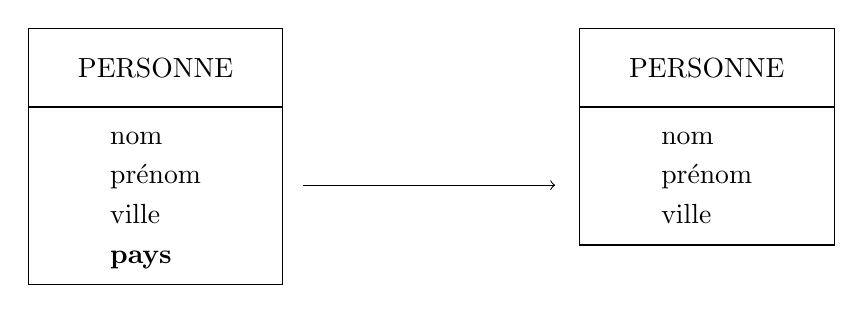
\begin{tikzpicture}
                \node [incolore, anchor=north west] at (0,0) {PERSONNE};
                \node [incolore, anchor=north west] at (0,-1) {\begin{tabular}{l}
                    nom \\
                    prénom \\
                    ville \\
                    \textbf{pays}
                \end{tabular}};

                \node [incolore, anchor=north west] at (7,0) {PERSONNE};
                \node [incolore, anchor=north west] at (7,-1) {\begin{tabular}{l}
                    nom \\
                    prénom \\
                    ville
                \end{tabular}};

                \draw[->] (3.5,-2) -- (6.7,-2);
            \end{tikzpicture}
        \end{center}
        L'attribut \textbf{pays} dépend de l'attribut ville qui n'est pas un identifiant. On doit donc le supprimer.
    \end{example}

\end{enumerate}



\end{itemize}















\section{Schéma conceptuel}










\subsection{Table}





\begin{itemize}



\item La \textbf{table} dans une base de données de type relationnel correspond à une entité du diagramme ERD.
\begin{itemize}
    \item elle est définie par un nom,
    \item ses colonnes sont ses attributs,
    \item ses lignes sont ses occurences.
\end{itemize}
\begin{center}
    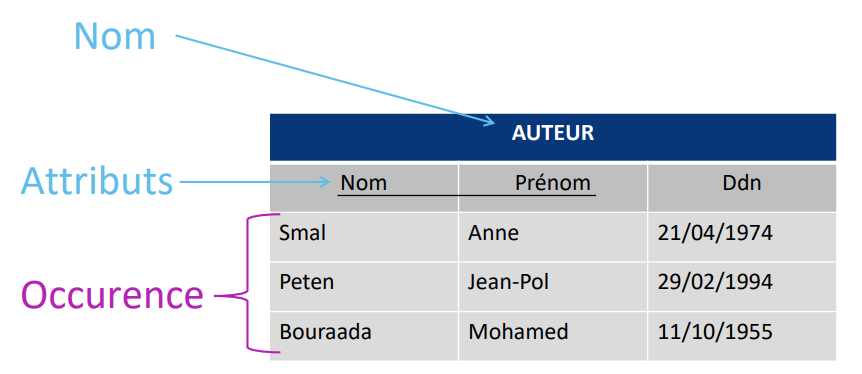
\includegraphics[width=0.5\textwidth]{../images/table01.PNG}
\end{center}



\item Valeur particulière dans une table: \texttt{null}, elle a 3 significations:
\begin{itemize}
    \item la valeur de l’attribut est inconnue pour certaines occurrences,
    \item l’attribut ne s’applique pas à certaines occurrences,
    \item certaines occurrences ne possèdent pas de valeur pour l’attribut.
\end{itemize}



\item \textbf{Remarque}: dans une BD relationnelle, l'ordre des lignes et des colonnes n'a pas d'importance.



\end{itemize}










\subsection{Clé primaire}





\begin{itemize}



\item La \textbf{clé primaire} est un attribut qui sert d'\textit{identifiant}.
\begin{itemize}
    \item un bon identifiant est un identifiant invariant,
    \item aucune clé primaire ne peut être \texttt{null},
    \item les identifiants composés sont rarement utilisés (on préfère un identifiant technique).
\end{itemize}



\item Pour stocker les relations entre les entités dans une table, on utilise des \textbf{clés étrangères}, c-à-d qu'on ajoute une colonne pour y stocker les clés primaires des autres tables.
\begin{center}
    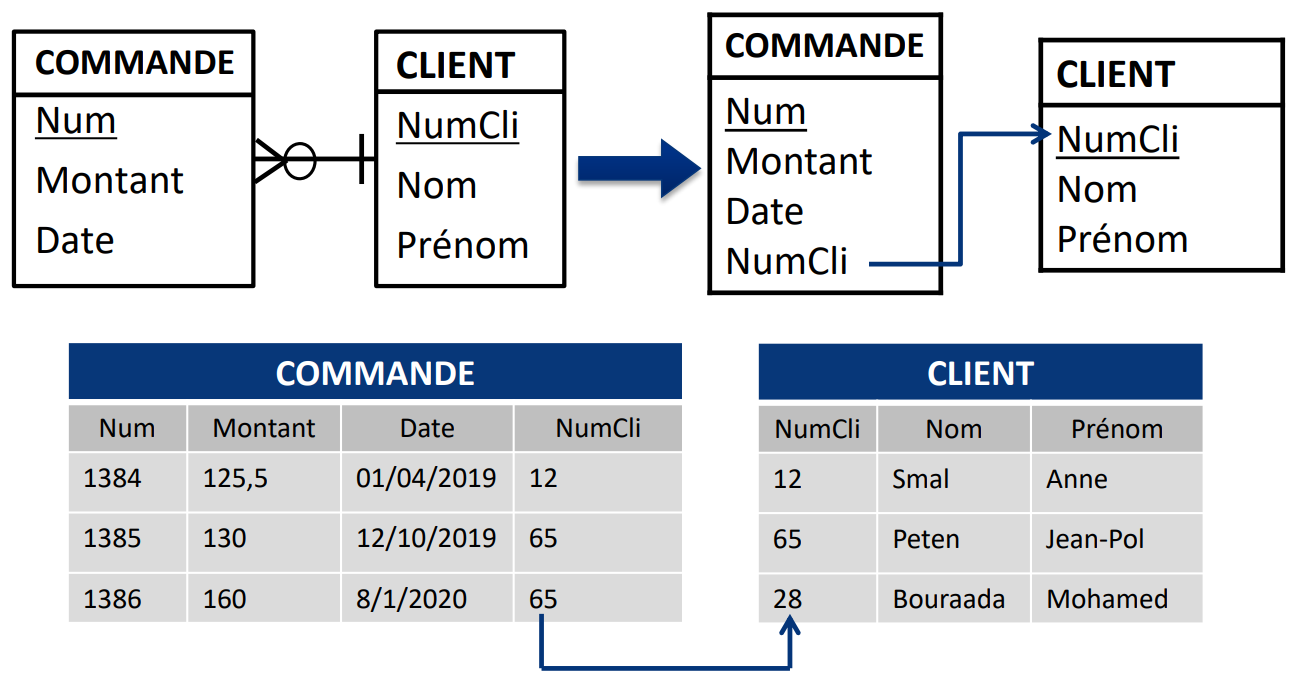
\includegraphics[width=0.70\textwidth]{../images/table02.PNG}
\end{center}



\item Où placer la clé étrangère ? On le fait en fonction des relations entre les entités:
\begin{itemize}
    \item relation 1-N $ \implies $ clé du côté N
    \item relation 1-1 $ \implies $ clé du côté 1
    \item relation 1-(0,1) $ \implies $ clé du côté (0,1)
    \item relation N-N $ \implies $ on crée une nouvelle entité qui représente la relation
\end{itemize}



\end{itemize}



Exemple relation N-N: \\
\begin{center}
    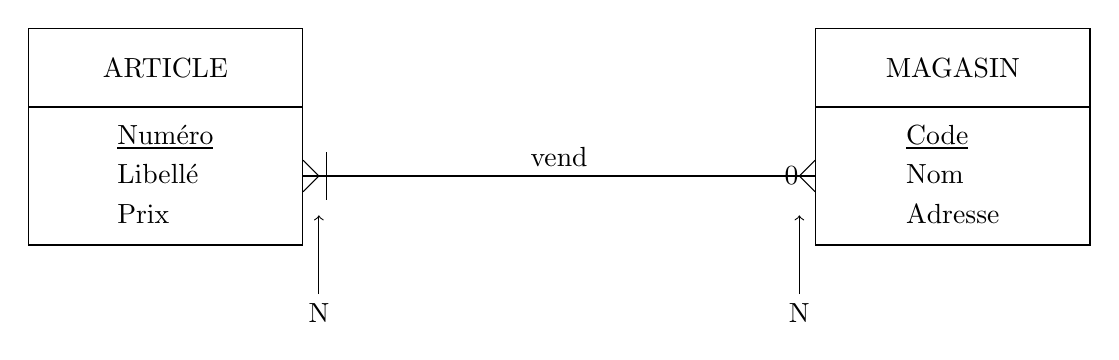
\begin{tikzpicture}

        %% entities
        \node () [incolore, anchor=north west, text width=3.25cm] at (0,0) {ARTICLE};
        \node (E1) [incolore, anchor=north west, text width=3.25cm] at (0,-1) {\begin{tabular}{l}
            \underline{Numéro} \\
            Libellé \\
            Prix
        \end{tabular}};

        \node () [incolore, anchor=north west, text width=3.25cm] at (10,0) {MAGASIN};
        \node (E2) [incolore, anchor=north west, text width=3.25cm] at (10,-1) {\begin{tabular}{l}
            \underline{Code} \\
            Nom \\
            Adresse
        \end{tabular}};


        %% relations
        \draw (E1) -- node[anchor=south]{vend} (E2);

        \draw ($(E1.east) + (0.2,0)$) -- ($(E1.east) + (0,0.2)$);
        \draw ($(E1.east) + (0.2,0)$) -- ($(E1.east) + (0,-0.2)$);
        \draw ($(E1.east) + (0.3,0.3)$) -- ($(E1.east) + (0.3,-0.3)$);

        \draw ($(E2.west) + (-0.2,0)$) -- ($(E2.west) + (0,0.2)$);
        \draw ($(E2.west) + (-0.2,0)$) -- ($(E2.west) + (0,-0.2)$);
        \node [] at ($(E2.west) + (-0.3,0)$) {0};


        %% notes
        \draw[->] ($(E1.east) + (0.2,-1.5)$) node[anchor=north]{N} -- ($(E1.east) + (0.2,-0.5)$);
        \draw[->] ($(E2.west) + (-0.2,-1.5)$) node[anchor=north]{N} -- ($(E2.west) + (-0.2,-0.5)$);

    \end{tikzpicture}

    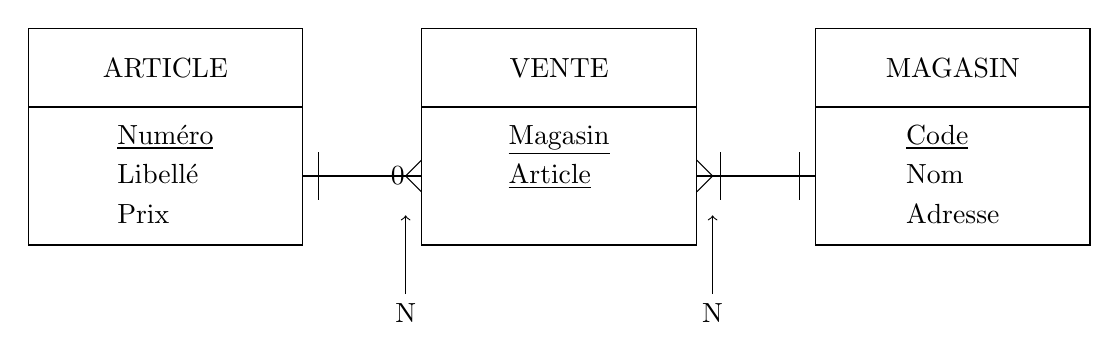
\begin{tikzpicture}

        %% entities
        \node () [incolore, anchor=north west, text width=3.25cm] at (0,0) {ARTICLE};
        \node (E1) [incolore, anchor=north west, text width=3.25cm] at (0,-1) {\begin{tabular}{l}
            \underline{Numéro} \\
            Libellé \\
            Prix
        \end{tabular}};

        \node () [incolore, anchor=north west, text width=3.25cm] at (10,0) {MAGASIN};
        \node (E2) [incolore, anchor=north west, text width=3.25cm] at (10,-1) {\begin{tabular}{l}
            \underline{Code} \\
            Nom \\
            Adresse
        \end{tabular}};

        \node () [incolore, anchor=north west, text width=3.25cm] at (5,0) {VENTE};
        \node (E3) [incolore, anchor=north west, text width=3.25cm] at (5,-1) {\begin{tabular}{l}
            \underline{Magasin} \\
            \underline{Article} \\
            \;
        \end{tabular}};


        %% relations
        \draw (E1) -- (E3);
        \draw (E3) -- (E2);

        \draw ($(E3.east) + (0.2,0)$) -- ($(E3.east) + (0,0.2)$);
        \draw ($(E3.east) + (0.2,0)$) -- ($(E3.east) + (0,-0.2)$);
        \draw ($(E3.east) + (0.3,0.3)$) -- ($(E3.east) + (0.3,-0.3)$);

        \draw ($(E3.west) + (-0.2,0)$) -- ($(E3.west) + (0,0.2)$);
        \draw ($(E3.west) + (-0.2,0)$) -- ($(E3.west) + (0,-0.2)$);
        \node [] at ($(E3.west) + (-0.3,0)$) {0};

        \draw ($(E1.east) + (0.2,0.3)$) -- ($(E1.east) + (0.2,-0.3)$);
        \draw ($(E2.west) + (-0.2,-0.3)$) -- ($(E2.west) + (-0.2,0.3)$);


        %% notes
        \draw[->] ($(E3.east) + (0.2,-1.5)$) node[anchor=north]{N} -- ($(E3.east) + (0.2,-0.5)$);
        \draw[->] ($(E3.west) + (-0.2,-1.5)$) node[anchor=north]{N} -- ($(E3.west) + (-0.2,-0.5)$);

    \end{tikzpicture}
\end{center}










\subsection{Schéma relationnel}





Pour convertir un schéma entité-relation en schéma relationnel, on ajoute les clés étrangères dans les entités et on trace une flèche qui part de la clé étrangère vers la clé primaire qu'elle représente.

Exemple:
\begin{center}
    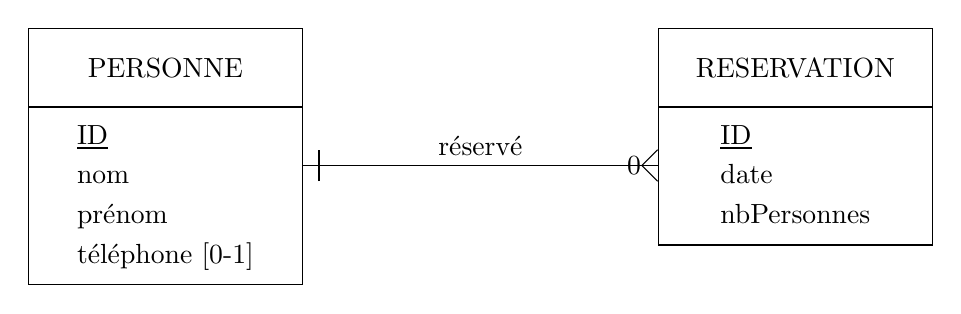
\begin{tikzpicture}

        \node () [incolore, anchor=north west, text width=3.25cm] at (0,0) {PERSONNE};
        \node (E1) [incolore, anchor=north west, text width=3.25cm] at (0,-1) {\begin{tabular}{l}
            \underline{ID} \\
            nom \\
            prénom \\
            téléphone [0-1]
        \end{tabular}};

        \node () [incolore, anchor=north west, text width=3.25cm] at (8,0) {RESERVATION};
        \node (E2) [incolore, anchor=north west, text width=3.25cm] at (8,-1) {\begin{tabular}{l}
            \underline{ID} \\
            date \\
            nbPersonnes
        \end{tabular}};


        \draw (3.5,-1.75) -- node[anchor=south]{réservé} (8,-1.75);
        \draw ($(3.5,-1.75) + (0.2,-0.2)$) -- ($(3.5,-1.75) + (0.2,0.2)$);

        \draw ($(8,-1.75) + (-0.2,0)$) -- ($(8,-1.75) + (0,0.2)$);
        \draw ($(8,-1.75) + (-0.2,0)$) -- ($(8,-1.75) + (0,-0.2)$);
        \node [] at ($(8,-1.75) + (-0.3,0)$) {0};

    \end{tikzpicture}

    \vspace{0.5cm}

    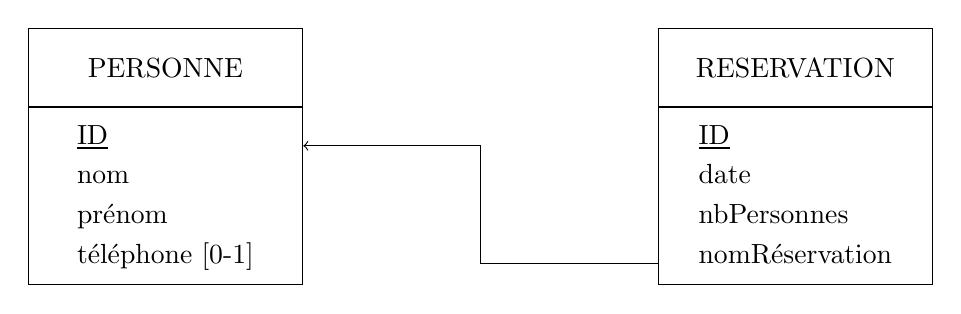
\begin{tikzpicture}

        \node () [incolore, anchor=north west, text width=3.25cm] at (0,0) {PERSONNE};
        \node (E1) [incolore, anchor=north west, text width=3.25cm] at (0,-1) {\begin{tabular}{l}
            \underline{ID} \\
            nom \\
            prénom \\
            téléphone [0-1]
        \end{tabular}};

        \node () [incolore, anchor=north west, text width=3.25cm] at (8,0) {RESERVATION};
        \node (E2) [incolore, anchor=north west, text width=3.25cm] at (8,-1) {\begin{tabular}{l}
            \underline{ID} \\
            date \\
            nbPersonnes \\
            nomRéservation
        \end{tabular}};


        \draw[->] (8,-3) -- (5.75,-3) -- (5.75,-1.5) -- (3.5,-1.5);

    \end{tikzpicture}
\end{center}

\textbf{Remarque:} dans certains cas, il faut ajouter \textbf{[0-1]} à côté de la clé étrangère si nécessaire. \\
Exemple:
\begin{center}
    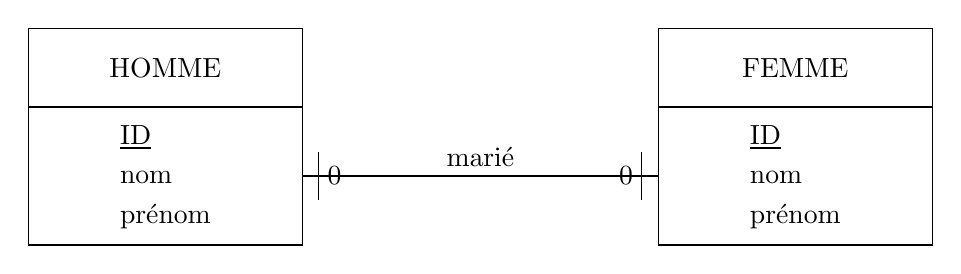
\begin{tikzpicture}
        
        \node () [incolore, anchor=north west, text width=3.25cm] at (0,0) {HOMME};
        \node (E1) [incolore, anchor=north west, text width=3.25cm] at (0,-1) {\begin{tabular}{l}
            \underline{ID} \\
            nom \\
            prénom \\
        \end{tabular}};

        \node () [incolore, anchor=north west, text width=3.25cm] at (8,0) {FEMME};
        \node (E2) [incolore, anchor=north west, text width=3.25cm] at (8,-1) {\begin{tabular}{l}
            \underline{ID} \\
            nom \\
            prénom \\
        \end{tabular}};


        \draw (E1) -- node[anchor=south]{marié} (E2);
        \draw ($(E1.east) + (0.2,0.3)$) -- ($(E1.east) + (0.2,-0.3)$);
        \draw ($(E2.west) + (-0.2,0.3)$) -- ($(E2.west) + (-0.2,-0.3)$);
        \node [] at ($(E1.east) + (0.4,0)$) {0};
        \node [] at ($(E2.west) + (-0.4,0)$) {0};

    \end{tikzpicture}

    \vspace{0.5cm}

    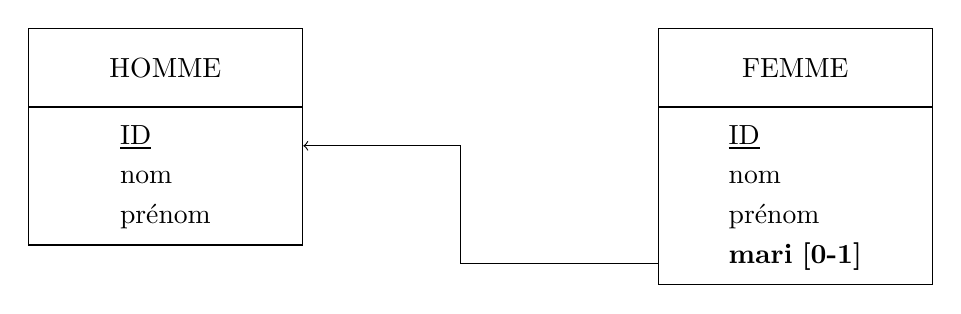
\begin{tikzpicture}
        
        \node () [incolore, anchor=north west, text width=3.25cm] at (0,0) {HOMME};
        \node (E1) [incolore, anchor=north west, text width=3.25cm] at (0,-1) {\begin{tabular}{l}
            \underline{ID} \\
            nom \\
            prénom \\
        \end{tabular}};

        \node () [incolore, anchor=north west, text width=3.25cm] at (8,0) {FEMME};
        \node (E2) [incolore, anchor=north west, text width=3.25cm] at (8,-1) {\begin{tabular}{l}
            \underline{ID} \\
            nom \\
            prénom \\
            \textbf{mari [0-1]}
        \end{tabular}};


        \draw[->] (8,-3) -- (5.5,-3) -- (5.5,-1.5) -- (3.5,-1.5);

    \end{tikzpicture}
\end{center}















\section{SQL}










\subsection{Base}





\begin{itemize}



\item Commande pour créer une base de données: \texttt{\textcolor{red}{CREATE} \textcolor{blue}{DATABASE} <nom\_db>;}



\item En SQL, la valeur \texttt{null} est une valeur spéciale. Par exemple, quand on crée une occurence et qu'on ne donne pas de valeur à un attribut optionnel, il prendra alors la valeur \texttt{null}.



\item Liste des types les plus communs:
\begin{itemize}
    \item \texttt{int} = entier
    \item \texttt{float} = nombre décimal,
    \item \texttt{varchar} = string/chaîne de caractères de taille variable
    \item \texttt{varchar2} = string pour laquelle: "" == \texttt{null}
    \item \texttt{date}, défaut = 1900-01-01
    \item \texttt{datetime}, défaut = 1900-01-01 00:00:00
\end{itemize}



\item Créer une table:
\begin{center}
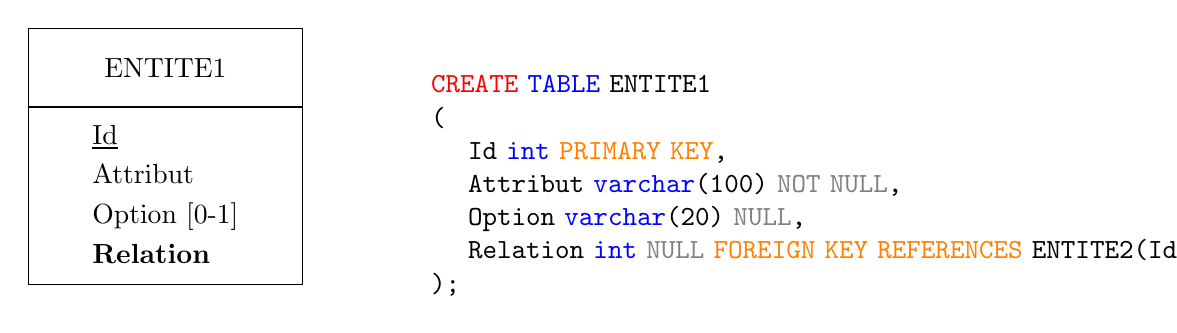
\begin{tikzpicture}
\node () [incolore, anchor=north west, text width=3.25cm] at (0,0) {ENTITE1};
\node (E1) [incolore, anchor=north west, text width=3.25cm] at (0,-1) {\begin{tabular}{l}
    \underline{Id} \\
    Attribut \\
    Option [0-1] \\
    \textbf{Relation}
\end{tabular}};

\node [anchor=north west, text width=9cm] at (5,0) {
\begin{Verbatim}[commandchars=\\\{\}]
\textcolor{red}{CREATE} \textcolor{blue}{TABLE} ENTITE1
(
    Id \textcolor{blue}{int} \textcolor{orange}{PRIMARY KEY},
    Attribut \textcolor{blue}{varchar}(100) \textcolor{gray}{NOT NULL},
    Option \textcolor{blue}{varchar}(20) \textcolor{gray}{NULL},
    \textbf{Relation} \textcolor{blue}{int} \textcolor{gray}{NULL} \textcolor{orange}{FOREIGN KEY REFERENCES} ENTITE2(Id),
);
\end{Verbatim}
};
\end{tikzpicture}
\end{center}



\end{itemize}










\subsection{Contraintes}





\begin{itemize}



\item Liste de contraintes qu'on peut donner aux attributs:
\begin{itemize}
    \item \texttt{\textcolor{gray}{NULL}} = attribut optionnel,
    \item \texttt{\textcolor{gray}{NOT NULL}} = attribut obligatoire,
    \item \texttt{\textcolor{orange}{PRIMARY KEY}} = l'attribut est une clé primaire,
    \item \texttt{\textcolor{orange}{FOREIGN KEY}} = l'attribut est une clé étrangère,
    \item \texttt{UNIQUE} = la valeur de l'attribut doit être différente pour chaque occurence,
    \item \texttt{DEFAULT <valeur>} = donne une valeur par défaut,
    \item \texttt{CHECK <condition>} = la valeur de l'attribut doit vérifier la condition donnée,
\end{itemize}
Exemple avec \texttt{check}:
\begin{Verbatim}[commandchars=\\\{\}]
\textcolor{red}{CREATE} \textcolor{blue}{TABLE} USER (
    UserName \textcolor{blue}{varchar}(63) PRIMARY KEY,
    Age \textcolor{blue}{int} CHECK (Age>=18),
);
\end{Verbatim}



\item Normalement, on ajoute les \textit{contraintes} après avoir déclarer l'attribut (ex: null, unique, etc.). Mais ce n'est pas obligatoire, on peut aussi ajouter des contraintes par après avec: \texttt{CONSTRAINT <nom\_contrainte> <contrainte>}. \\
Exemples:
\begin{itemize}
    \item \texttt{\textcolor{red}{CONSTRAINT} <nom\_contrainte1> UNIQUE email},
    \item \texttt{\textcolor{red}{CONSTRAINT} <nom\_contrainte2> \texttt{CHECK} (Age>=18 AND Pays='Belgium')},
    \item \texttt{\textcolor{red}{CONSTRAINT} <nom\_contrainte3> \texttt{\textcolor{gray}{NOT NULL}} prenom},
    \item \texttt{\textcolor{red}{CONSTRAINT} <nom\_contrainte4> \texttt{\textcolor{orange}{PRIMARY KEY}} Id},
    \item \texttt{\textcolor{red}{CONSTRAINT} <nom\_contrainte5> \texttt{\textcolor{orange}{FOREIGN KEY}} IdVille \texttt{\textcolor{orange}{REFERENCES}} VILLE (IdVille)},
    \item \texttt{\textcolor{red}{CONSTRAINT} <nom6> \texttt{\textcolor{orange}{FOREIGN KEY}} (IdPart1, IdPart2) \texttt{\textcolor{orange}{REFERENCES}} ENTITE (IdPart1, IdPart2)},
\end{itemize}


Exemple avec la création d'une table:
\begin{center}
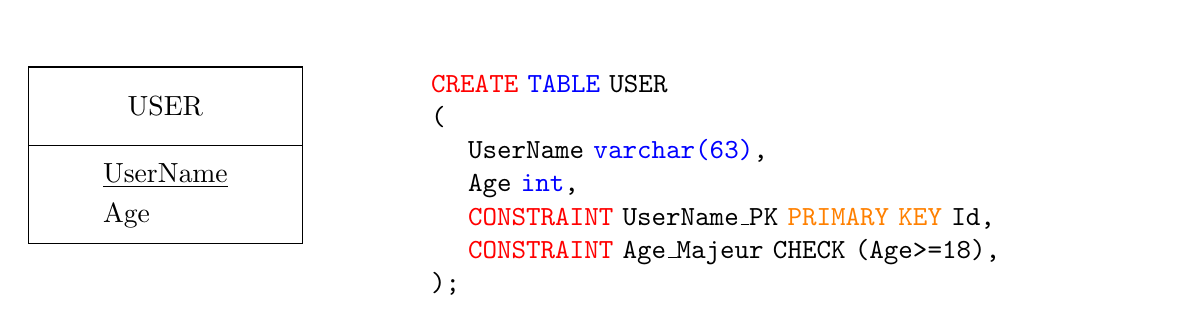
\begin{tikzpicture}
\node () [incolore, anchor=north west, text width=3.25cm] at (0,0) {USER};
\node (E1) [incolore, anchor=north west, text width=3.25cm] at (0,-1) {\begin{tabular}{l}
    \underline{UserName} \\
    Age
\end{tabular}};

\node [anchor=north west, text width=9cm] at (5,0.5) {
\begin{Verbatim}[commandchars=\\\{\}]
\textcolor{red}{CREATE} \textcolor{blue}{TABLE} USER
(
    UserName \textcolor{blue}{varchar(63)},
    Age \textcolor{blue}{int},
    \textcolor{red}{CONSTRAINT} UserName\_PK \textcolor{orange}{PRIMARY KEY} Id,
    \textcolor{red}{CONSTRAINT} Age\_Majeur CHECK (Age>=18),
);
\end{Verbatim}       
};
\end{tikzpicture}
\end{center}



\end{itemize}










\subsection{Modifier une table}





\begin{itemize}



\item Supprimer une table: \texttt{\textcolor{red}{DROP} \textcolor{blue}{TABLE} <nom\_table>;}.



\item Vider une table: \texttt{\textcolor{red}{TRUNCATE} \textcolor{blue}{TABLE} <nom\_table>;}.



\item Renommer une table: \texttt{\textcolor{red}{EXEC} \textcolor{blue}{sp\_rename} <nom\_table>, <nouveau\_nom>;}.



\item Renommer une colonne:\\
\texttt{\textcolor{red}{EXEC} \textcolor{blue}{sp\_rename} '<table>.<ancien\_nom>', '<nouveau\_nom>', 'COLUMN';}
\begin{example}
    \texttt{\textcolor{red}{EXEC} \textcolor{blue}{sp\_rename} 'USER.UserName', 'NomUtilisateur', 'COLUMN';}
\end{example}



\item Pour modifier la structure d'une table, on doit utiliser la commande: \texttt{\textcolor{red}{ALTER} \textcolor{blue}{TABLE} <nom\_table>\\ <instruction>;}. Comme instruction, on peut mettre:
\begin{itemize}
    \item \texttt{\textcolor{red}{ADD} <colonne> <type>;}
    \begin{example}
        \texttt{\textcolor{red}{ALTER} \textcolor{blue}{TABLE} USER \textcolor{red}{ADD} DateCreationCompte date;}
    \end{example}
    \item \texttt{\textcolor{red}{ALTER COLUMN} <colonne> <type>;}
    \begin{example}
        \texttt{\textcolor{red}{ALTER} \textcolor{blue}{TABLE} USER \textcolor{red}{ALTER COLUMN} DateCreationCompte datetime \textcolor{gray}{NOT NULL};}
    \end{example}
    \item \texttt{\textcolor{red}{DROP} <colonne>;} \texttt{\textcolor{red}{DROP COLUMN} <colonne>;}
    \begin{example}
        \texttt{\textcolor{red}{ALTER} \textcolor{blue}{TABLE} USER \textcolor{red}{DROP} DateCreationCompte, Age;}
    \end{example}
\end{itemize}



\end{itemize}










\subsection{Manipulation des données}





\begin{itemize}



\item Ajouter des données: \texttt{\textcolor{red}{INSERT} INTO USER (UserName, Age) \textcolor{blue}{VALUES} ("Greg", 50000);}



\item Modifier des données: \texttt{\textcolor{red}{UPDATE} USER \textcolor{red}{SET} Age=852 \textcolor{blue}{WHERE} UserName="Greg";}



\item Supprimer des données: \texttt{\textcolor{red}{DELETE} \textcolor{blue}{FROM} USER \textcolor{blue}{WHERE} UserName="Greg";}



\item Obtenir des données: \texttt{\textcolor{red}{SELECT} <colonnes> \textcolor{blue}{FROM} <table>;} \\
On peut aussi ajouter des conditions avec: \texttt{where}, et ordonner les valeurs avec: \texttt{order by} (on peut ajouter: \texttt{asc}, ou: \texttt{desc} pour préciser si on trie par ordre croissant ou décroissant).



\item Opérateurs:
\begin{itemize}
    \item logiques: $\sim$ (not), \&, |, $\wedge$ (xor), NOT, AND, OR
    \item math: \; +, \; -, \; *, \; /, \; \%
    \item comparaison: \; =, \; >, \; <, \; >=, \; <=, \; <>, \; !=, \; !>, \; !<
\end{itemize}



\item L'opérateur \texttt{LIKE} permet de comparer des string/chaînes de caractères.
\begin{example}
    \begin{itemize}

        \item \texttt{\textcolor{red}{SELECT} * \textcolor{blue}{FROM} USER \textcolor{blue}{WHERE} UserName LIKE 'Gre\textcolor{purple}{\%}';}\\
        cette commande sélectionne toutes les occurences de \texttt{user} dont le nom d'utilisateur commence par \textit{gre} (ex: gre, greg, gregoire, etc.).

        \item \texttt{\textcolor{red}{SELECT} * \textcolor{blue}{FROM} USER \textcolor{blue}{WHERE} UserName LIKE 'gre\textcolor{purple}{\_}';}\\
        cette commande donne les utilisateurs qui commencent par \textit{gre} et qui ont un caractère en plus (ex: greg, grec, etc.).

    \end{itemize}
\end{example}



\item Pour filtrer des éléments \texttt{null}, on ne peut pas utiliser la comparaison = ou !=. Il faut utiliser \texttt{is} ou \texttt{is not}.
\begin{example}
    \texttt{\textcolor{red}{SELECT} * \textcolor{blue}{FROM} USER \textcolor{blue}{WHERE} Age IS NOT \textcolor{gray}{NULL};}
\end{example}



\end{itemize}










\subsection{Fonctions}





\begin{itemize}



\item Fonctions simples:
\begin{center}
    \begin{tabular}{lll}
        \texttt{\textcolor{red}{UPPER}('string')}               & $ \implies $ & \texttt{STRING} \\
        \texttt{\textcolor{red}{LOWER}('STRING')}               & $ \implies $ & \texttt{string} \\
        \texttt{\textcolor{red}{CONCAT}('str1', 'str2')}        & $ \implies $ & \texttt{str1str2} \\
        \texttt{\textcolor{red}{LEN}('string')}                 & $ \implies $ & \texttt{6} \\
        \texttt{\textcolor{red}{REPLACE}('string', 'tri', 'o')} & $ \implies $ & \texttt{song} \\
        \texttt{\textcolor{red}{ROUND}(123.321, 2)}             & $ \implies $ & \texttt{123.32} \\
        \texttt{\textcolor{red}{LEFT}('string', 3)}             & $ \implies $ & \texttt{str} \\
        \texttt{\textcolor{red}{LTRIM}('string', 3)}            & $ \implies $ & \texttt{ing} \\
    \end{tabular}
\end{center}



\item Fonctions de groupes:
\begin{center}
    \begin{tabular}{lll}
        \texttt{\textcolor{red}{AVG}}   & = & moyenne \\
        \texttt{\textcolor{red}{COUNT}} & = & nombre \\
        \texttt{\textcolor{red}{MAX}}   & = & maximum \\
        \texttt{\textcolor{red}{MIN}}   & = & minimum \\
        \texttt{\textcolor{red}{SUM}}   & = & somme \\
    \end{tabular}
\end{center}



\end{itemize}










\subsection{Groupes}





\begin{itemize}



\item On crée des groupes avec: \texttt{GROUP BY}. Exemple:
\begin{itemize}
    \item Table:
    \begin{center}
        \begin{tabular}{|c|c|} \hline
            & lettre \\ \hline
            1 & 'a' \\ \hline
            2 & 'b' \\ \hline
            3 & 'a' \\ \hline
            4 & 'b' \\ \hline
            5 & 'a' \\ \hline
        \end{tabular}
    \end{center}
    \item SQL: \texttt{\textcolor{red}{SELECT} lettre \textcolor{blue}{FROM} TABLE \textcolor{blue}{GROUP BY} lettre;}
    \item Résultat:
    \begin{center}
        \begin{tabular}{|c|c|} \hline
            & lettre \\ \hline
            1 & 'a' \\ \hline
            2 & 'b' \\ \hline
        \end{tabular}
    \end{center}
\end{itemize}



\item Pour filtrer les groupes, on n'utilise pas \texttt{WHERE} mais \texttt{HAVING}. Exemple:
\begin{itemize}
    \item SQL: \texttt{\textcolor{red}{SELECT} lettre, \textcolor{red}{COUNT}(*) \textcolor{blue}{FROM} TABLE \textcolor{blue}{GROUP BY} lettre \textcolor{blue}{HAVING} \textcolor{red}{COUNT}(*) = 3;}
    \item Résultat:
    \begin{center}
        \begin{tabular}{|c|c|} \hline
            & lettre \\ \hline
            1 & 'a' \\ \hline
        \end{tabular}
    \end{center}
\end{itemize}



\end{itemize}










\subsection{Requêtes imbriquées}





Opérateurs pour les requêtes imbriquées:
\begin{center}
     \begin{tabular}{lll}
        IN     & $ \implies $ & vrai si l'élément est dans les valeurs renvoyées par le select imbriqué \\
        ANY    & $ \implies $ & vrai si la condition est vérifié pour au moins 1 ligne \\
        ALL    & $ \implies $ & vrai si la condition est vérifié pour toutes les lignes \\
        EXISTS & $ \implies $ & vrai si au moins 1 ligne est renvoyée \\
     \end{tabular}
\end{center}





Exemples:
\begin{itemize}



\item Objectif: prendre les id et les noms des clients qui ont une facture.
\begin{itemize}
    \item SQL: \texttt{\textcolor{red}{SELECT} Id, Nom \textcolor{blue}{FROM} CLIENT \textcolor{blue}{WHERE} Id \textcolor{blue}{IN} ( \textcolor{red}{SELECT} Client \textcolor{blue}{FROM} FACTURE );}
    \item Résultat:
    \begin{center}
        \begin{tabular}{|l|l|l|} \hline
            & Id & Nom \\ \hline
            1 & 1 & Alice \\ \hline
            2 & 2 &   Bob \\ \hline
            3 & 3 & Chris \\ \hline
        \end{tabular}
    \end{center}
\end{itemize}



\item Objectif: ...
\begin{itemize}
    \item SQL: \texttt{\textcolor{red}{SELECT} Id, Nom \textcolor{blue}{FROM} CLIENT \textcolor{blue}{WHERE} Id > \textcolor{blue}{ALL} ( \textcolor{red}{SELECT} Client \textcolor{blue}{FROM} FACTURE );}
    \item Résultat:
    \begin{center}
        \begin{tabular}{|l|l|l|} \hline
            & Id & Nom \\ \hline
            1 & 4 & David \\ \hline
        \end{tabular}
    \end{center}
\end{itemize}



\end{itemize}










\subsection{Jointures}





\begin{itemize}



\item Les jointures servent à lier des colonnes de tables différentes. Exemple:
\begin{itemize}
    \item Tables:
    \begin{center}
        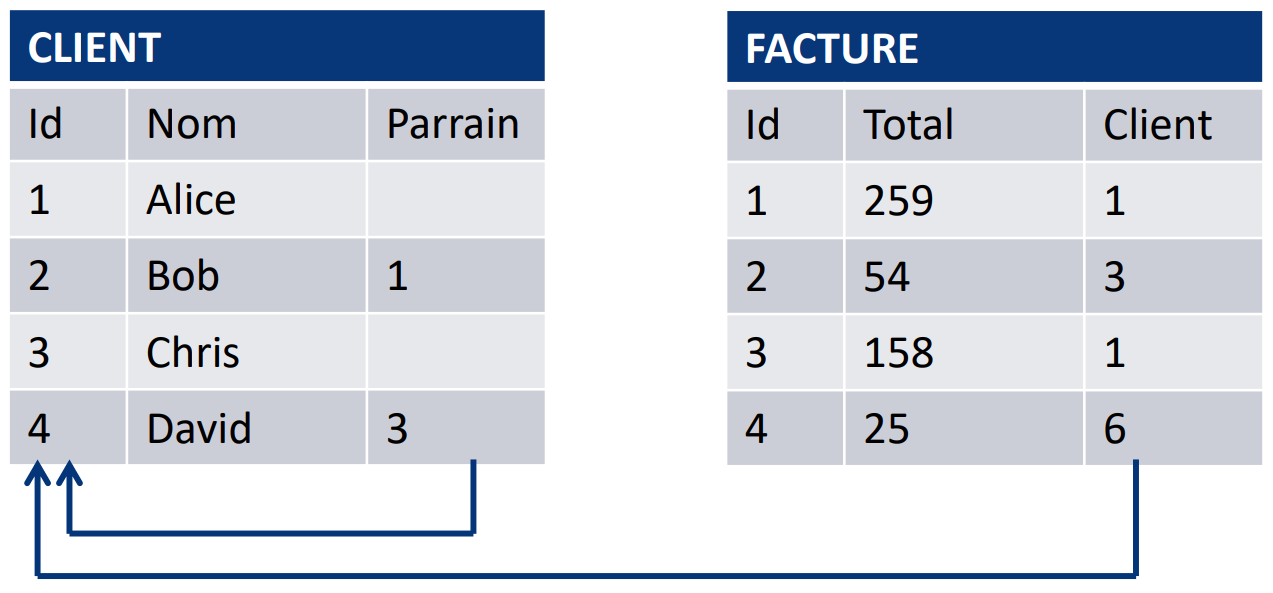
\includegraphics[width=0.5\textwidth]{../images/jointures-01.PNG}
    \end{center}
    \item SQL: \texttt{\textcolor{red}{SELECT} * \textcolor{blue}{FROM} CLIENT C \textcolor{red}{JOIN} FACTURE F \textcolor{red}{ON} C.Id = F.Client;}
    \item Résultat:
    \begin{center}
        \begin{tabular}{|l|l|l|l|l|l|l|} \hline
            & Id & Nom & Parrain & Id & Total & Client \\ \hline
            1 &  1 & Alice & NULL & 1 & 259 & 1 \\ \hline
            2 &  3 & Chris & NULL & 2 &  54 & 3 \\ \hline
            3 &  1 & Alice & NULL & 3 & 158 & 1 \\ \hline
            4 &  2 & Bob   & 1    & 4 &  25 & 2 \\ \hline
        \end{tabular}
    \end{center}
    \item SQL: \texttt{\textcolor{red}{SELECT} Nom, Total \textcolor{blue}{FROM} CLIENT C \textcolor{red}{JOIN} FACTURE F \textcolor{red}{ON} C.Id = F.Client;}
    \item Résultat:
    \begin{center}
        \begin{tabular}{|l|l|l|} \hline
            & Nom & Total \\ \hline
            1 & Alice & 259 \\ \hline
            2 & Chris &  54 \\ \hline
            3 & Alice & 158 \\ \hline
            4 &   Bob &  25 \\ \hline
        \end{tabular}
    \end{center}
\end{itemize}



\item Liste des jointures normales:
\begin{itemize}


    %% INNER JOIN
    \item \texttt{SELECT C.Id, Nom FROM CLIENT C \textcolor{red}{INNER JOIN} FACTURE F ON C.Id = F.Client;}
    \begin{center}
        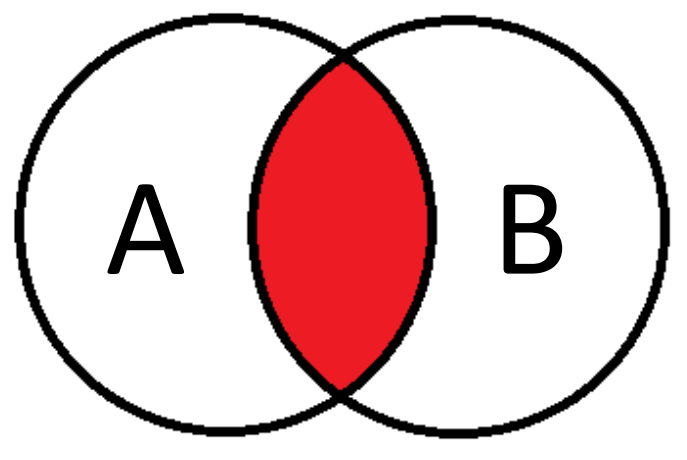
\includegraphics[width=0.25\textwidth]{../images/inner-join-01.PNG}
    \end{center}
    \begin{center}
        \begin{tabular}{|l|l|l|l|l|l|l|} \hline
            & \multicolumn{3}{l|}{CLIENT} & \multicolumn{3}{l|}{FACTURE} \\ \hline
            & Id & Nom & Parrain & Id & Total & Client \\ \hline
            \rowcolor{orange!30}
            1 & 1 & Alice &   & 1 & 259 & 1 \\ \hline
            \rowcolor{orange!30}
            2 & 1 & Alice &   & 3 & 158 & 1 \\ \hline
            3 & 2 &   Bob & 1 &   &     &   \\ \hline
            \rowcolor{orange!30}
            4 & 3 & Chris &   & 2 &  54 & 3 \\ \hline
            5 & 4 & David & 3 &   &     &   \\ \hline
            6 &   &       &   & 4 &  25 & 6 \\ \hline
        \end{tabular}
    \end{center}


    %% FULL OUTER JOIN
    \item \texttt{SELECT C.Id, Nom FROM CLIENT C \textcolor{red}{FULL OUTER JOIN} FACTURE F ON C.Id = F.Client;}
    \begin{center}
        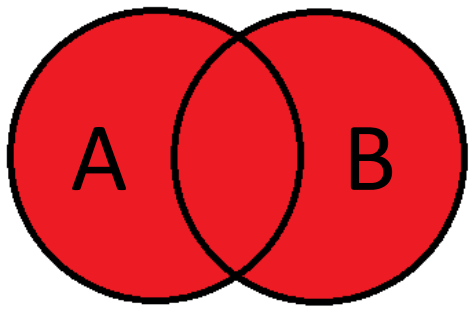
\includegraphics[width=0.25\textwidth]{../images/full-outer-join-01.PNG}
    \end{center}
    \begin{center}
        \begin{tabular}{|l|l|l|l|l|l|l|} \hline
            & \multicolumn{3}{l|}{CLIENT} & \multicolumn{3}{l|}{FACTURE} \\ \hline
            & Id & Nom & Parrain & Id & Total & Client \\ \hline
            \rowcolor{orange!30}
            1 & 1 & Alice &   & 1 & 259 & 1 \\ \hline
            \rowcolor{orange!30}
            2 & 1 & Alice &   & 3 & 158 & 1 \\ \hline
            \rowcolor{orange!30}
            3 & 2 &   Bob & 1 &   &     &   \\ \hline
            \rowcolor{orange!30}
            4 & 3 & Chris &   & 2 &  54 & 3 \\ \hline
            \rowcolor{orange!30}
            5 & 4 & David & 3 &   &     &   \\ \hline
            \rowcolor{orange!30}
            6 &   &       &   & 4 &  25 & 6 \\ \hline
        \end{tabular}
    \end{center}


    %% LEFT JOIN
    \item \texttt{SELECT C.Id, Nom FROM CLIENT C \textcolor{red}{LEFT JOIN} FACTURE F ON C.Id = F.Client;}
    \begin{center}
        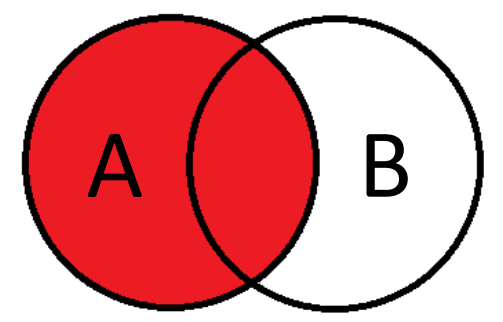
\includegraphics[width=0.25\textwidth]{../images/left-join-01.PNG}
    \end{center}
    \begin{center}
        \begin{tabular}{|l|l|l|l|l|l|l|} \hline
            & \multicolumn{3}{l|}{CLIENT} & \multicolumn{3}{l|}{FACTURE} \\ \hline
            & Id & Nom & Parrain & Id & Total & Client \\ \hline
            \rowcolor{orange!30}
            1 & 1 & Alice &   & 1 & 259 & 1 \\ \hline
            \rowcolor{orange!30}
            2 & 1 & Alice &   & 3 & 158 & 1 \\ \hline
            \rowcolor{orange!30}
            3 & 2 &   Bob & 1 &   &     &   \\ \hline
            \rowcolor{orange!30}
            4 & 3 & Chris &   & 2 &  54 & 3 \\ \hline
            \rowcolor{orange!30}
            5 & 4 & David & 3 &   &     &   \\ \hline
            6 &   &       &   & 4 &  25 & 6 \\ \hline
        \end{tabular}
    \end{center}


    %% RIGHT JOIN
    \item \texttt{SELECT C.Id, Nom FROM CLIENT C \textcolor{red}{RIGHT JOIN} FACTURE F ON C.Id = F.Client;}
    \begin{center}
        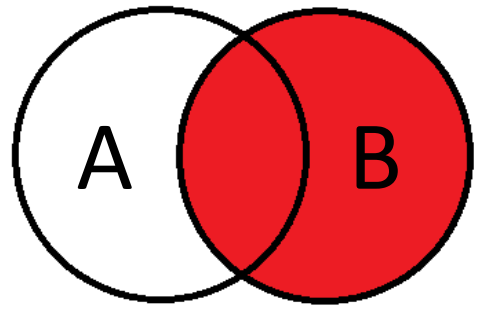
\includegraphics[width=0.25\textwidth]{../images/right-join-01.PNG}
    \end{center}
    \begin{center}
        \begin{tabular}{|l|l|l|l|l|l|l|} \hline
            & \multicolumn{3}{l|}{CLIENT} & \multicolumn{3}{l|}{FACTURE} \\ \hline
            & Id & Nom & Parrain & Id & Total & Client \\ \hline
            \rowcolor{orange!30}
            1 & 1 & Alice &   & 1 & 259 & 1 \\ \hline
            \rowcolor{orange!30}
            2 & 1 & Alice &   & 3 & 158 & 1 \\ \hline
            3 & 2 &   Bob & 1 &   &     &   \\ \hline
            \rowcolor{orange!30}
            4 & 3 & Chris &   & 2 &  54 & 3 \\ \hline
            5 & 4 & David & 3 &   &     &   \\ \hline
            \rowcolor{orange!30}
            6 &   &       &   & 4 &  25 & 6 \\ \hline
        \end{tabular}
    \end{center}


    %% FULL OUTER JOIN
    \item \texttt{SELECT C.Id, Nom FROM CLIENT C \textcolor{red}{FULL OUTER JOIN} FACTURE F ON C.Id = F.Client} \\ \texttt{\textcolor{blue}{WHERE} C.Id IS NULL OR F.Client IS NULL;}
    \begin{center}
        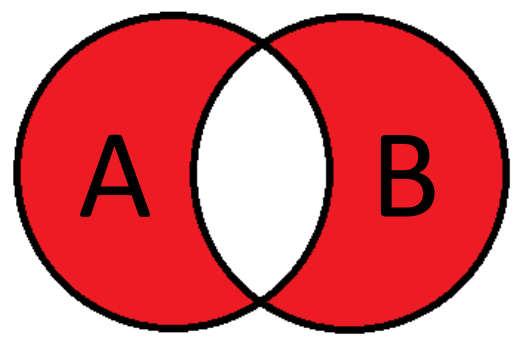
\includegraphics[width=0.25\textwidth]{../images/full-outer-join-02.PNG}
    \end{center}
    \begin{center}
        \begin{tabular}{|l|l|l|l|l|l|l|} \hline
            & \multicolumn{3}{l|}{CLIENT} & \multicolumn{3}{l|}{FACTURE} \\ \hline
            & Id & Nom & Parrain & Id & Total & Client \\ \hline
            1 & 1 & Alice &   & 1 & 259 & 1 \\ \hline
            2 & 1 & Alice &   & 3 & 158 & 1 \\ \hline
            \rowcolor{orange!30}
            3 & 2 &   Bob & 1 &   &     &   \\ \hline
            4 & 3 & Chris &   & 2 &  54 & 3 \\ \hline
            \rowcolor{orange!30}
            5 & 4 & David & 3 &   &     &   \\ \hline
            \rowcolor{orange!30}
            6 &   &       &   & 4 &  25 & 6 \\ \hline
        \end{tabular}
    \end{center}


    %% LEFT JOIN
    \item \texttt{SELECT C.Id, Nom FROM CLIENT C \textcolor{red}{LEFT JOIN} FACTURE F ON C.Id = F.Client} \\ \texttt{\textcolor{blue}{WHERE} F.Client IS NULL;}
    \begin{center}
        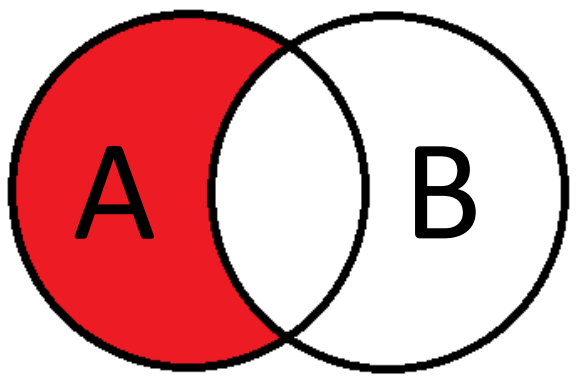
\includegraphics[width=0.25\textwidth]{../images/left-join-02.PNG}
    \end{center}
    \begin{center}
        \begin{tabular}{|l|l|l|l|l|l|l|} \hline
            & \multicolumn{3}{l|}{CLIENT} & \multicolumn{3}{l|}{FACTURE} \\ \hline
            & Id & Nom & Parrain & Id & Total & Client \\ \hline
            1 & 1 & Alice &   & 1 & 259 & 1 \\ \hline
            2 & 1 & Alice &   & 3 & 158 & 1 \\ \hline
            \rowcolor{orange!30}
            3 & 2 &   Bob & 1 &   &     &   \\ \hline
            4 & 3 & Chris &   & 2 &  54 & 3 \\ \hline
            \rowcolor{orange!30}
            5 & 4 & David & 3 &   &     &   \\ \hline
            6 &   &       &   & 4 &  25 & 6 \\ \hline
        \end{tabular}
    \end{center}


    %% RIGHT JOIN
    \item \texttt{SELECT C.Id, Nom FROM CLIENT C \textcolor{red}{RIGHT JOIN} FACTURE F ON C.Id = F.Client} \\ \texttt{\textcolor{blue}{WHERE} C.Id IS NULL;}
    \begin{center}
        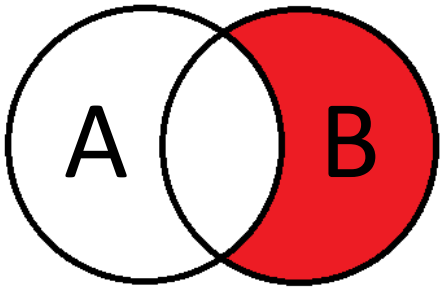
\includegraphics[width=0.25\textwidth]{../images/right-join-02.PNG}
    \end{center}
    \begin{center}
        \begin{tabular}{|l|l|l|l|l|l|l|} \hline
            & \multicolumn{3}{l|}{CLIENT} & \multicolumn{3}{l|}{FACTURE} \\ \hline
            & Id & Nom & Parrain & Id & Total & Client \\ \hline
            1 & 1 & Alice &   & 1 & 259 & 1 \\ \hline
            2 & 1 & Alice &   & 3 & 158 & 1 \\ \hline
            3 & 2 &   Bob & 1 &   &     &   \\ \hline
            4 & 3 & Chris &   & 2 &  54 & 3 \\ \hline
            5 & 4 & David & 3 &   &     &   \\ \hline
            \rowcolor{orange!30}
            6 &   &       &   & 4 &  25 & 6 \\ \hline
        \end{tabular}
    \end{center}


\end{itemize}



\item Jointure sur les colonnes de même nom:
\begin{itemize}
    \item SQL: \texttt{\textcolor{red}{SELECT} colonnes \textcolor{blue}{FROM} tableA A \textcolor{red}{NATURAL JOIN} tableB B;}
    \item Tables:
    \begin{center}
        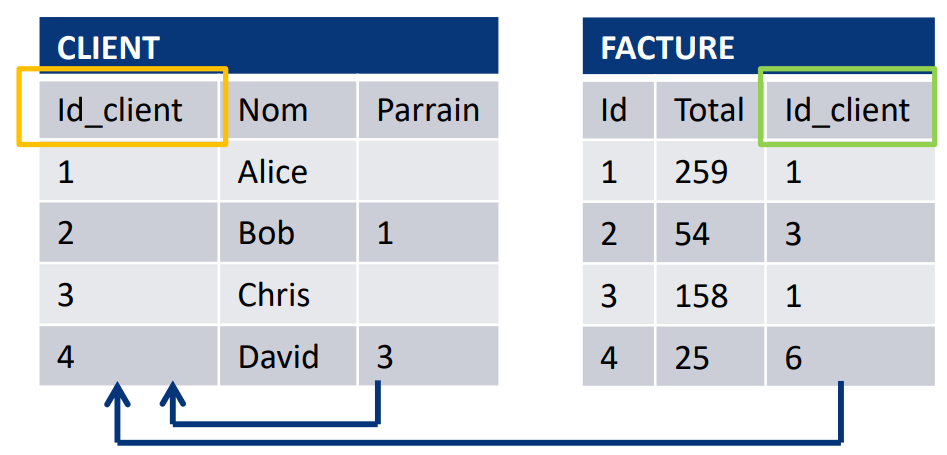
\includegraphics[width=0.5\textwidth]{../images/natural-join-01.PNG}
    \end{center}
\end{itemize}



\item Faire correspondre chaque ligne de A avec chaque ligne de B
\begin{itemize}
    \item SQL: \texttt{\textcolor{red}{SELECT} colonnes \textcolor{blue}{FROM} tableA A \textcolor{red}{CROSS JOIN} tableB B}
    \item Tables:
    \begin{center}
        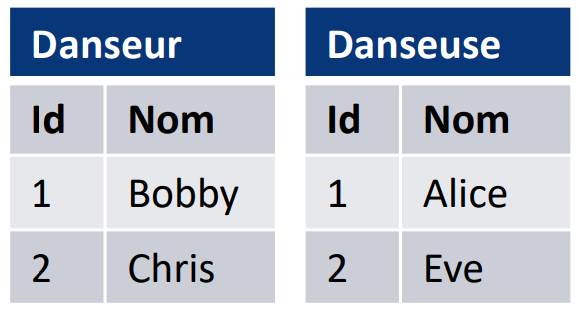
\includegraphics[width=0.25\textwidth]{../images/cross-join-01.PNG}
    \end{center}
    \item Résultat:
    \begin{center}
        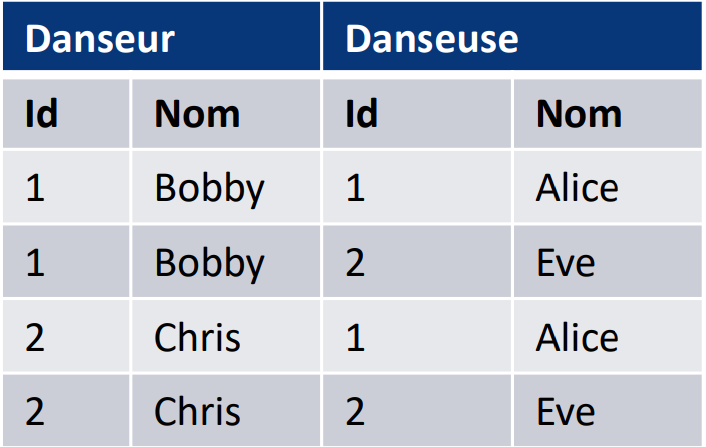
\includegraphics[width=0.30\textwidth]{../images/cross-join-02.PNG}
    \end{center}
\end{itemize}



\item Jointure pour une table qui a une clé étrangère vers elle-même:
\begin{itemize}
    \item SQL: \texttt{SELECT \textcolor{orange}{cli}.Id, \textcolor{orange}{cli}.Nom, \textcolor{green}{par}.Nom AS Parrain} \\
    \texttt{FROM CLIENT \textcolor{orange}{cli}} \\
    \texttt{INNER JOIN CLIENT \textcolor{green}{par}} \\
    \texttt{ON \textcolor{orange}{cli}.Parrain = \textcolor{green}{par}.Id}
    \item Tables:
    \begin{center}
        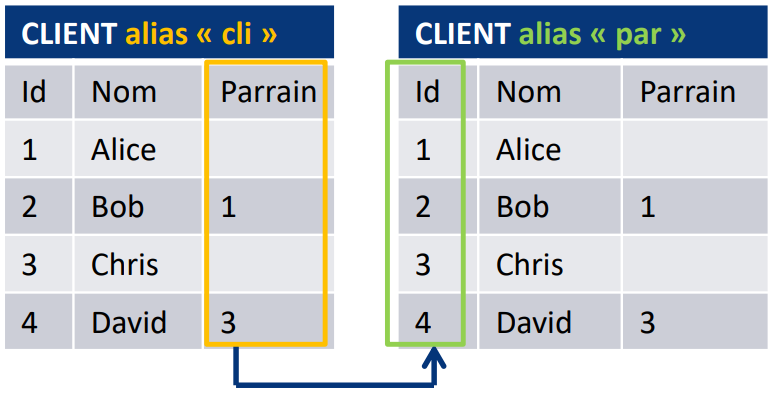
\includegraphics[width=0.5\textwidth]{../images/self-join-01.PNG}
    \end{center}
    \item Résultats:
    \begin{center}
        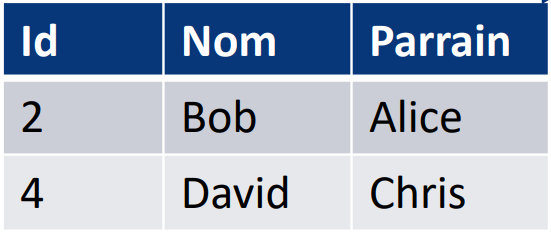
\includegraphics[width=0.25\textwidth]{../images/self-join-02.PNG}
    \end{center}
\end{itemize}



\end{itemize}




















\end{document}
